% $\circledcirc \_ \circledcirc$

\section{Waves}

\noindent D'alambert equation:
$$\frac{\partial^2y}{\partial t^2} = v^2 \frac{\partial^2y}{\partial x^2}$$

\noindent Intensity:
$$I \propto A^2$$
$$I_{1+2} \propto |A_1e^{ia_1} + A_2e^{ia_2}|^2 = A_1^2 + A_2^2 + 2A_1A_2cos(a_1 - a_2)$$

\noindent Versione esponenziale:
$$y(x, t) = Ae^{i(kx - \omega t + \phi)}$$

\section{Double - Slit}

\noindent L'alternanza delle fasce luminose e scure avviene quando i due cammini sono uguali o hanno una differenza di \textit{k} volte la lunghezza d'onda $\lambda$.
$$\delta = k\Delta = kd\sin(\theta) \sim kxd / L$$

\noindent Dove:
\begin{itemize}
    \item $k$ = Numero d'onda
    \item $\Delta$ = Differenza di cammino
    \item $\theta$ = Angolo formato dal centro (primo ordine)
    \item $x$ = Distanza dal centro (primo ordine)
    \item $d$ = Distanza tra gli slit
    \item $L$ = Distanza dello schermo dagli slit
\end{itemize}

L'intensità in questo caso risulterà essere:
$$I_{1+2} \propto 2A^2(1 + cos(k\Delta))$$

\section{Photoelectric}

\noindent Dato un circuito abbiamo che indipendentemente dall'intensità, non riusciamo a strappare elettroni da una superficie metallica, quando però la frequenza arriva ad un certo punto, avviene passaggio di corrente, e a questo punto essa sarà proporzionale all'intensità dell'onda.

\section{De Broglie}

$$\begin{array}{l c r}
    E = h\nu & p = h\lambda & E=p^2 / 2m
\end{array}$$

\noindent In pratica possiamo sostituire nell'esponenziale i termini di energia e otteniamo:
$$\psi_p(x, t) = Ae^{i \frac{2\pi}{h} (px - Et)}$$

\noindent Provando però ad eseguire queste sostituzioni, scopriamo che non rispettano più l'equazioni di d'Alambert, le evidenze sperimentali ci portano ad ottenere una nuova riformulazione:
$$i\hbar \frac{\partial}{\partial t}\psi_p(\vec{x}, t) = \frac{p^2}{2m}\psi_p(\vec{x}, t) = E\psi_p(\vec{x}, t) = -\frac{\nabla^2}{2m}\psi_p(\vec{x}, t)$$

\section{Eigen - Stuff}

\paragraph{Stato fisico:}
In un sistema fisico (che può essere una o più particelle), lo stato fisico del sistema è descritto da un vettore NORMALIZZATO $\ket{\psi(t)}$ chiamato funzione d'onda. Se il $\braket{\psi(t)|\psi(t)} = 1$ allora è normalizzato.

\paragraph{Osservabile:}
Le quantità misurabili di un sistema (posizione, energia, momento angolare, ecc.) sono chiamate \textit{osservabili}, esse sono descritte dagli operatori Hermitiani. Esiste la \textit{Principio di Corrispondenza} che sarebbe la promozione da 'quantità fisica' a 'operatore'.

\paragraph{Operatore hermitiano:} 
Operatore (matrice) che agendo sullo stato fisico (funzione d'onda $\psi$) permette di ottenere un'autovalore. L'operatore è hermitiano se $\hat{A^{\dagger}} = \hat{A}$, ovvero se è uguale alla sua \textbf{TRASPOSTA - CONIUGATA}.

\paragraph{Autovalore:}
Valore associato all'operatore, rappresenta la quantità misurabile, di fatto è uguale all'azione dell'operatore in quel specifico caso. Questo significa che l'azione dell'operatore su uno stato fisico, lo porta a collassare in un singolo valore (la misura).

\paragraph{Autostato / Autovettore:}
Stato $\bra{l}$ che descrive lo stato originale $\ket{\psi}$ dopo l'applicazione di $\hat{A}$. Se $\psi$ non è uno auto-stato dell'operatore originariamente, allora questo verrà scomposto in una combinazione lineare di auto-stati dell'operatore.

\paragraph{Probabilità:}
Se ad uno stato fisico applichiamo un'operatore, otterremo la corrispettiva combinazione di autovalori e autostati. L'autostato sarà normalizzato. La probabilità di ottenere esattamente l'autovalore come risultato della misura, dipenderà da quanto lo stato fisico prima e dopo overlappano:
$$\rho(\lambda_l) = |\braket{l|\psi}|^2$$
Dal momento che la probabilità di uno auto-stato dipende dal suo modulo quadro, la fase non avrà effetto sulla probabilità, dunque due auto-stati saranno considerati uguali anche se hanno una fase diversa.

\paragraph{Ripetibilità:}
Se applichiamo un'operatore su uno stato fisico generico e lo facciamo collassare in uno auto-stato, se ripetiamo la misurazione \textit{'Immediately afterwards'} (lo stato non ha tempo di cambiare a causa della time evolution) il risultato non cambierà e otterremo l'autovalore con probabilità del 100\%. Questo perchè dopo la prima applicazione, lo stato $\ket{\psi}$ è collassato in una combinazione lineare di autostati dell'operatore, quindi riapplicare l'operatore porterà ad ottenere un fattore di scala (autovalore $\lambda$) che si integra perfettamente con la nuova base di autostati.

\paragraph{Expectation values (media):}
In pratica applichiamo l'operatore $\hat{A}$ su $\psi$, portandolo in una combinazione di autostati intermedi. Subito dopo calcoliamo l'overlap della combinazione di autostati con lo stato originale eseguendo il $\braket{\psi|l}$. Rieseguendo lo stesso calcolo N volte, otteniamo che in media la combinazione di autovalori risultanti sarà uguale a $\braket{A}$, ovvero la media.
$$\braket{A} = \braket{\psi|A|\psi}$$

\section{Schr\"{o}dinger}

$$i\hbar\frac{d}{dt}\ket{\psi(t)} = H\ket{\psi(t)}$$

\noindent H è l'hamiltoniana del sistema, ovvero l'insieme delle energie. Di seguito sono riportati operatori importanti.

$$\hat{x} = x$$ $$\hat{p} = -i\hbar\vec{\nabla}$$

\paragraph{Commutazioni:}
La formula generica dice che $[A, B] = AB - BA$, se questo è uguale a 0, allora i due operatori commutano. Nel caso di posizione e quantità di moto, non commutano. Dimostrazione nel principio di indeterminazione di Heisenberg.

\paragraph{Calcolo commutatore posizione quantità di moto:}
Applichiamo il commutatore $[A, B]$ su una $f(x)$ qualsiasi, e vediamo quanto vale:
$$-i\hbar\left[x, \frac{\partial}{\partial x}\right] f(x) = -i\hbar\left[x\frac{\partial f(x)}{\partial x} - \frac{\partial (xf(x))}{\partial x}\right]$$
Applicando la regola del prodotto di derivate $f'(xy) = yf'(x) + xf'(y)$ abbiamo che: 
$$-i\hbar\left( \cancel{x\frac{\partial f(x)}{\partial x}} - \cancel{x \frac{\partial f(x)}{\partial x}} - f(x)\frac{\partial x}{\partial x}\right) = i\hbar f(x)$$
Quindi abbiamo un termine moltiplicativo rimanente uguale a $i\hbar$.

\paragraph{Normalizzazione usando t:}
$$\braket{\psi(t)|\vec{x}}\braket{\vec{x}|\psi(t)} = |\psi(\vec{x}, t)|^2 \equiv \rho(\vec{x}, t)$$

\section{Time evolution}

L'hamiltoniana è intrinsecamente time-indipendent dal momento che sia l'operatore spazio che l'operatore quantità di moto lo sono. Questo significa che possiamo cercare delle soluzioni particolari che abbiano lo spazio e il tempo fattorizzato:
$$\phi(\vec{x}, t) = \phi(\vec{x})f(t)$$
Sostituiamo nell'equazione di Schr\"{o}dinger originale:
$$i\hbar\frac{\partial}{\partial t}\phi(\vec{x})f(t) = H\phi(\vec{x})f(t)$$
Molitplichiamo entrambi i termini per $1 / \phi(\vec{x}, t)$:
$$\frac{1}{\phi(\vec{x})f(t)}i\hbar\frac{\partial}{\partial t}\phi(\vec{x})f(t) = \frac{1}{\phi(\vec{x})f(t)}H\phi(\vec{x})f(t)$$
Dato che a sinistra la derivata agisce solo su $f(t)$, mentre a destra agisce solo $\phi(\vec{x})$:
$$\frac{1}{f(t)}i\hbar\frac{\partial}{\partial t}f(t) = \frac{1}{\phi(\vec{x})}H\phi(\vec{x})$$
Possiamo dire che dato che entrambi i lati dipendono solo da un tipo di variabile per volta, allora avremo che questi due termini saranno uguali ad un valore E:
$$\frac{1}{f(t)}i\hbar\frac{\partial}{\partial t}f(t) = E \longrightarrow f(t) \propto e^{-iEt/\hbar}$$
Mentre l'equazione classica dipendente solo da x, rimane la stessa. Quindi la soluzione totale, sarà una funzione di x per una fase di t:
$$\phi(\vec{x}, t) = \phi(\vec{x})e^{-iEt/\hbar}$$

\noindent Questo ci porta a poter calcolare un generico stato $\psi$ con stato iniziale $\braket{\psi(0)}$ come:
$$\ket{\psi(t)} = \sum_{i}e^{-iE_it/\hbar} \ket{\phi_i(0)} \braket{\phi_i(0)|\psi(0)}$$

\noindent E credo che possiamo quindi risolvere il problema come:
$$\ket{\psi(t)} = e^{-iHt/\hbar}\ket{\psi(0)}$$

\paragraph{ESERCIZIO DALLA PROVA:} A quantum system evolves with a time-indipendent Hamiltonian $\hat{H}$ and at $t = 0$ is in state $\ket{\psi(0)} = (\ket{1} + \ket{2}) / \sqrt{2}$, where $\ket{n}$ are energy eigenstates with $\hat{H}\ket{n} = E_n\ket{n}$.

\noindent What is the probability that the system will be found in the initial state at time $T > 0$?

\vspace{15pt}

\noindent Per calcolare la probabilità usiamo:
$$P = \big|\braket{\Psi(0)|\Psi(t)}\big|^2$$
Sostituendo i valori delle $\Psi$ otteniamo:
$$\braket{\Psi_0|\Psi_t} = \bigg\langle\frac{\ket{1} + \ket{2}}{\sqrt{2}}\bigg|\frac{e^{-iE_1T/\hbar}\ket{1} + e^{-iE_2T/\hbar}\ket{2}}{\sqrt{2}}\bigg\rangle$$
Calcoliamo le varie combinazioni ricordando che $\braket{a|a} = 1$, mentre $\braket{a|b} = 0$
$$\braket{\Psi_0|\Psi_t} = \frac{1}{2}\left( e^{-iE_1T/\hbar} + e^{-iE_2T/\hbar} \right)$$
Ora possiamo trasformare tutto in coseni con la seguente formula:
$$e^{iA} + e^{iB} = 2e^{i(A+B)/2} \cos\left(\frac{A-B}{2}\right)$$
$$P = \bigg|\frac{1}{\cancel{2}}\cancel{2}e^{-i(E_1+E_2)T/2\hbar}\cos\left( \frac{(E_1-E_2)T}{2\hbar}\right)\bigg|^2$$
Eliminando la parte immaginaria perchè tanto con il valore assoluto scompare:
$$P = \cos^2\left( \frac{(E_1-E_2)T}{2\hbar} \right)$$
Sapendo che esiste la relazione:
$$\cos^2(a) = \frac{1+cos(2a)}{2}$$
$$P = \frac{1}{2}\left(1 + \cos\left( \frac{(E_1 - E_2)T}{\hbar} \right)\right)$$

\section{Uncertainty}

È possibile avere una base ortonormale composta da autostati comuni a due operatori (ovvero che commutano). Per esempio:
$$A\ket{\lambda_k, \beta_k} = \lambda_k\ket{\lambda_k, \beta_k} \text{ and } B\ket{\lambda_k, \beta_k} = \beta_k\ket{\lambda_k, \beta_k}$$

\noindent Questo significa che applicando uno dei due operatori, otteniamo comunque un autovalore e un autostato sempre. Se invece i due operatori non commutano NON possiamo trovare una base comune ad entrambi.

\paragraph{Standard - Deviation:}
Concetto importante, ovvero la differenza che esiste tra l'operatore e l'expectation value di quest'ultimo su uno stato generico $\psi$. Immagino che su uno stato generico (non autostato), il valore che si ottiene di discosta tanto più sia difficile rappresentare con una base di autostati questa situazione:
$$\Delta\hat{x} \equiv \hat{x} - \braket{\psi|\hat{x}|\psi}$$
Mentre la varianza, non è altro che il quadrato della deviazione standard:
$$(\Delta x)^2 \equiv \braket{\psi|(\Delta \hat{x})^2|\psi} = \braket{\psi|\hat{x}^2|\psi} - \braket{\psi|\hat{x}|\psi}^2$$
Il modo in cui puoi derivarlo è sviluppando il quadrato:
$$\Delta \hat{x} ^ 2 = (\hat{x} - \braket{\hat{x}})^2 = \hat{x}^2 + \braket{\hat{x}}^2 - 2\braket{\hat{x}}\hat{x}$$
Dato che $\braket{\hat{x}}$ è un valore reale, quando metti tutto dentro al calcolo $\braket{\psi|X|\psi}$, la costante può uscire, lasciandoti con solo il risultato trovato prima.

\paragraph{Schwarz inequality:}
Molto straight - forward $\longrightarrow \braket{v|v}\braket{w|w}\geq|\braket{v|w}|^2$, in teoria dovrebbe significare che la varianza minima che uno può ottenere è il quadrato del prodotto delle varianze.

\paragraph{Heisenberg Uncertainty Principle:}
Possiamo usare questa ugualianza per riscrivere tutto in termini di $x$ e $p$.
$$(\Delta x)^2(\Delta p_x)^2 \equiv \braket{\psi|(\Delta \hat{x})^2|\psi}\braket{\psi|(\Delta \hat{p_x})^2|\psi} \geq |\braket{\psi|\Delta\hat{x}\Delta\hat{p}_x|\psi}|^2$$

\paragraph{General decomposition commutatori:}
$$AB = [A, B] / 2 + \{A, B\} / 2$$
Possiamo usarla per risolvere finalmente il problema precedente:
$$(\Delta x)^2(\Delta p_x)^2 \geq \frac{1}{4}\Big|\braket{\psi|[\Delta\hat{x}, \Delta\hat{p}_x]|\psi} + \braket{\psi|\{\Delta\hat{x}, \Delta\hat{p}_x\}|\psi}\Big|^2$$
Una volta che proviamo a scomporre il $(a + b)^2 = a^2 + b^2 + 2ab$, si può usare MOLTA matematica per dimostrare che la parte $[A,B]$ è puramente immaginaria, mentre $\{A, B\}$ è puramente reale, e che il prodotto di parte reale pura per parte immaginaria pura ci darà un nuovo numero immaginario. Prendendo i valori assoluti li eliminerà, lasciando solo la componente con il commutatore $[A,B]$.
$$(\Delta x)^2(\Delta p_x)^2 \geq \frac{1}{4}\Big|\braket{\psi|[\hat{x}, \hat{p}_x]|\psi}\Big|^2$$
Dal capitolo prima sappiamo che il commutatore posizione e quanittà di moto è uguale ad $\hbar$.
$$\Delta x\Delta p_x \geq \frac{\hbar}{2}$$


\section{Current density}

\paragraph{Continuity equation:}
Ci dice che la carica totale è conservata, al massimo si può spostare:
$$\frac{\partial \rho (\vec{x}, t)}{\partial t} = -\vec{\nabla}\vec{J}(\vec{x}, t)$$
Se proviamo ad integrare nello spazio i due termini, ovvero fare il
$\int_{V}d^3x$
dove tra l'altro tutti i termini in funzione di $(t)$ escono, otteniamo per il primo termine:
$$\frac{dQ}{dt}$$
Mentre per il secondo termine usando il teorema della divergenza, il quale dice che \textit{'Il flusso in uscita attraverso una superficie chiusa è uguale alla divergenza all'interno del volume'}:
$$-\int_{S}\vec{J}(\vec{x}, t) \cdot d\vec{S} = -I$$
Quello che si può fare è calcolare quanto vale:
$$\frac{\partial \rho}{\partial t} = \frac{\partial}{\partial t}(\psi^*\psi) = -\vec{\nabla} \cdot \left\{ \frac{\hbar}{2mi} \left( \psi^*\vec{\nabla}\psi - \psi\vec{\nabla}\psi^* \right)\right\}$$
Quindi prendendo la prima equazione di continuità:
$$\vec{J}(\vec{x}, t) = \frac{\hbar}{2mi}\left( \psi^*\vec{\nabla}\psi - \psi\vec{\nabla}\psi^* \right)$$

\section{Potential step: E $> V_0$}

In ogni esercizio legato alle barriere di densità dovrà essere rispettata la condizione di continuità di $f(x)$ e $f'(x)$. Questo è dovuto al fatto che usando la seguente equazione di Schr\"{o}dinger, una discontinuità renderebbe le varie derivate di forme diverse, e quindi i due lati dell'equazione non uguali:
$$\frac{d^2\psi(x)}{dx^2}=-\frac{2m}{\hbar^2}(E-V(x))\psi(x)$$
In questo caso avremo che l'energia della particella sarà maggiore dell'ostacolo, avremo quindi due diverse funzioni (prima e dopo) e la differenza tra le due sta nel coefficiente moltiplicativo:
$$\text{I) } \frac{d^2\psi(x)}{dx^2}=-\frac{2mE}{\hbar^2}\psi_{\text{I}}(x)$$
$$\text{II) } \frac{d^2\psi(x)}{dx^2}=-\frac{2m(E-V(x))}{\hbar^2}\psi_{\text{II}}(x)$$
Noi possiamo raccogliere appunto dal lato destro dell'equazione tutto ciò che non è $\psi$, ottenendo:
$$k \equiv \sqrt{2mE} / \hbar$$
$$q \equiv \sqrt{2m(E-V_0)} / \hbar$$
Ora possiamo usare delle funzioni di prova che descrivono un'onda stazionaria e cercare di trovare un risultato:
$$\psi_{\text{I}} = Ae^{ikx} + Be^{-ikx}$$
$$\psi_{\text{II}} = Ce^{iqx} + De^{-iqx}$$
Da qui ricaviamo che se applicassimo l'hamiltoniana a una delle $\psi$ otterremmo che risolvendo i calcoli abbiamo l'autovalore uguale a:
$$E_{\text{I}} = \frac{\hbar^2k^2}{2m}$$
$$E_{\text{II}} = \frac{\hbar^2q^2}{2m}+V_0$$
Dal momento che sappiamo che c'è continuità tra le due equazioni, possiamo calcolare quanto vale il tutto a 0. Nota che l'equazione (II) non ha più il termine D, questo perchè assumiamo che dalla barriera non arrivi più nulla.
$$\psi_{\text{I}}=A+B = \psi_{\text{II}}=C$$
$$\psi'_{\text{I}}=ik(A-B) = \psi'_{\text{II}}=iqC$$
Nella parte delle derivate, è solo la derivata dell'esponenziale di $e^{ikx}$. Questo non ci permette di quantificare esattamente i coefficienti, ma ci permette di trovare una loro relazione, sostituendo C con A + B nell'equazione delle derivate, otteniamo:
$$\frac{B}{A} = \frac{k-q}{k+q}$$
Usando questo risultato e sostituendo in C = A + B il valore di B con quello che abbiamo appena trovato otteniamo:
$$\frac{C}{A}=\frac{2k}{k+q}$$
Dall'equazione delle correnti possiamo ottenere una migliore comprensione di cosa è A, B e C. (Guarda com'è l'equazione della corrente, la cosa importante è che facendo $\psi^*\psi$ avrai l'ampiezza al quadrato):
$$\frac{\hbar k}{m}(|A|^2-|B|^2) = J_{\text{in}} - J_{\text{refl}}$$
Puoi fare la stessa cosa con $\psi_{\text{II}}$ e otterrai:
$$\frac{\hbar q}{m}|C|^2 = J_{\text{trans}}$$
Questi sono i valori che possiamo usare per calcolare i coefficienti di trasmissione e riflessione, fai semplicemente il rapporto dei 2:
$$\text{Refl} = \frac{|B|^2}{|A|^2}$$
$$\text{Trans} = \frac{q}{k}\frac{|C|^2}{|A|^2}$$

\paragraph{Conclusioni:}
Nel caso quantistico ci sarà sempre un minimo di riflessione, anche se questa tenderà a zero per differenza di energia molto grandi. Nel caso classico invece è vero o falso.

\section{Potential step: E $< V_0$}

Consideriamo la stessa identica cosa, ma ora il potenziale è maggiore dell'energia della particella. In questo caso però quando calcoliamo 'g' (la vecchia 'q'), dovremo raccogliere un meno per rendere la radice risolvibile, questo significa che otterremo la seguente equazione:
$$\psi_{\text{II}}(x) = Ce^{-gx}+De^{gx}$$
Questo però significa che se $D \neq 0$ allora per $x \rightarrow \infty$, $\psi$ diverge. Questo ci porta a mettere $D = 0$. Se $D=0$, allora significa che il coefficiente di trasmissione sarà nullo. Questo significa che la particella non verrà trasmessa attraverso lo step, ma la sua funziona d'onda non svanirà istantaneamente, avrà una rapida diminuzione.
Se ricalcoliamo i rapporti tra B/A = 1 e C/A = 0 rimpiazzando $iq \rightarrow g$ otterremo che dentro lo step, abbiamo un decadimento esponenziale della funzione d'onda oramai diventata reale. Puoi anche dimostrarlo con la densità di corrente se vuoi.

\paragraph{Caso con $V_0 \rightarrow \infty$:} Se consideriamo un potenziale che tende ad $\infty$, allora la propagazione tenderà a zero, rendendo discontinua l'equazione. È tutto corretto, ricorda che la penetrazione con potenziale assunto ad infinito è uguale a 0.

\section{Effetto tunnel}

Immaginiamo invece ora di avere uno step di dimensioni non infinite, ma di un certa larghezza L e altezza $V_0$ e tutto attorno 0. Ora avremo 3 equazioni diverse che descrivono come si comporta la particella:
$$\psi_{\text{I}} = Ae^{ikx} + Be^{-ikx}$$
$$\psi_{\text{II}} = Fe^{-gx} + De^{gx}$$
$$\psi_{\text{III}} = Ce^{ikx}$$
Dove ricordiamo che $k$ è il valore con solo $E$, mentre $g$ è il valore con $V_0 - E$. Non lo scrivo, ma poniamo le \textbf{condizioni di continuità} in entrambi i lati con sia la funzione base che la derivata. Per risolvere le equazioni è molto semplice usare come sistema di riferimento l'inizio della barriera a $-L/2$ e la fine a $L/2$. Possiamo quindi ricavare il valore di $F$ e $D$ usando le equazioni della parte destra (per semplicità, così c'è solo C e non A + B), e sommandole tra loro e sottraendole otterremo D e F. Ricorda che per eseguire questo calcolo è utile dividere la derivata della continuità di destra per $g$.

\paragraph{Considerazioni:} Abbiamo una decrescita esponenziale all'interno della barriera, ma poi una successiva ricomparsa al suo termine SE la barriera è abbastanza stretta, per larghezze che tendono ad infinito, il sistema si comporta come nel caso dello step. Ricorda che anche l'altezza influenza la forza di attenuazione. Ci sono parecchi calcoli con sinusoidi iperboliche che skippo, sono usati per il calcolo della densità di corrente. Sappi che per $gL << 1$ avremo una trasmissione di circa 1.

\section{WKB}

E se il potenziale della barriera non fosse costante? Beh possiamo riscrivere l'equazione di partenza con $V(x)$ anzichè $V(0)$.
$$\frac{d^2\psi(x)}{dx^2}=k^2(x)\psi(x), \text{ dove } k(x) \equiv \sqrt{2m(V(x) - E)} / \hbar$$
Si dimostra che sostituendo il tutto con la seguente formula si ottiene una fedele approssimazione nel caso in cui il potenziale è una funzione che è \textit{slowly varying}. Questo è possibile dimostrarlo derivando 2 volte il tutto:
$$\psi(x) \sim \psi(x_0)\exp\left( -\int_{x_0}^{x} dx'k(x') \right)$$
Quindi, nel caso in cui abbiamo effettivamente un'ostacolo tra $x_1$ e $x_2$, possiamo scrivere che:
$$\psi(x_2) \sim \psi(x_1) \exp \left( - \int_{x_1}^{x_2} dx \sqrt{2m(V(x) - E)}/\hbar \right)$$
Questo semplifica di molto il calcolo della trasmissione, perchè se il risultato è semplicemente il rapporto, allora:
$$t(E) \sim \frac{|\psi(x_2)|^2}{|\psi(x_1)|^2} \sim \exp \left( - 2 \int_{x_1}^{x_2} dx \sqrt{2m(V(x) - E)}/\hbar \right)$$
Il due che c'è dentro alla parentesi è dovuto al quadrato che viene portato dentro all'esponenziale. Come cross-check puoi controllare che funziona anche per la barriera piatta.

\section{$\alpha$ - decay}

Uno dei possibili utilizzi della WKB. Sappiamo che dentro al nucleo ci sono delle forze di attrazione, tali per cui la particella $\alpha$ non riesce a liberarsi. Superata questa barriera, la particella subirebbe la repulsione Couloumbiana legata alla repulsione tra 2 particelle cariche positivamente. In tutto questo stiamo trascurando l'effetto degli elettroni su questi 2 nuclei.

Questo significa che il nucleo $\alpha$ possiede una certa energia E non sufficiente a superare l'attrazione nucleare, ma sufficiente a trovarsi a qualche femtometro di distanza, dove con la propria energia riesce a matchare l'energia di repulsione Couloumbiana. Questo significa che la particella dovrà 'tunnelare' attraverso questa curva.
$$V(r) = \frac{Z_1Z_2e^2}{4\pi\varepsilon_0r}$$ 
$$t(E) = \exp \left[ -\frac{2\sqrt{2*4m_p}}{\hbar} \int_{r_1}^{r_2} dr\sqrt{V(r) - E} \right]$$ 
Questa formula è letteralmente la formula di soluzione dell'effetto tunnel usando la WKB con la formula del potenziale sostituito.

\begin{figure}[ht]
	\centering
	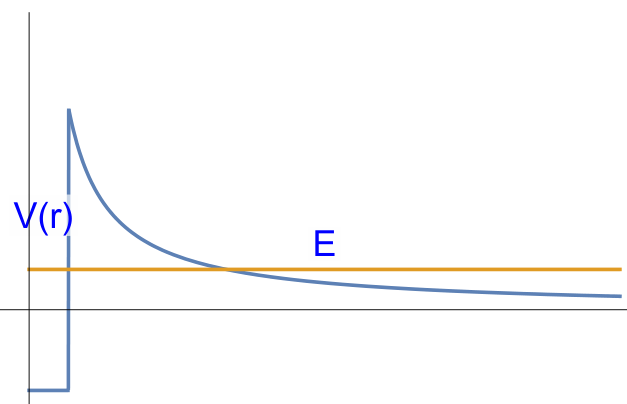
\includegraphics[width=.5\textwidth]{../images/Screenshot 2025-02-17 144907.png}
	\caption{Potenziale $\alpha$-decay}
	\label{fig:alpha_decay}
\end{figure}

\paragraph{Sviluppo:}
Possiamo definire altri valori, come il punto di massima energia, il punto in cui l'energia della particella $\alpha$ e il potenziale Couloumbiano si ugualiano. Possiamo inoltre ricordare che il raggio del nucleo scala all'incirca con questa forma: $R \sim Z_1^{1/3}$. Viene inoltre introdotta anche la vita media, come $\ln{\tau} \propto -\ln t(E)$.
Un'importante considerazione è il fatto che l'espulsione di questi nuclei di He è più propensa per nuclei più leggeri, ma c'è da ricordare che nella realtà questi nuclei hanno mooolta più energia nei nuclei più pesanti, garantendo quindi che l'effetto sia più propenso negli elementi più pesanti.

\section{Cold emission}
Un altro caso di utilizzo è la cold emission usato nell'STM (Scanning Tunnelling Microscope). In questo caso però la barriera da superare è infinita, nel senso che senza un aiuto esterno, l'attrazione del materiale, chiamata \textit{work-function} $\Phi$ è costante nello spazio, come anche l'energia dell'elettrone, che però è minore di $\Phi$.

Quando però un campo elettrico esterno viene applicato, 'richiamando' l'elettrone, il potenziale $\Phi$ viene schiacciato verso il basso creando un potenziale triangolare, che, usando la WKB possiamo risolvere, trovando il punto dove $V(x) = \Phi + E - |e|\mathcal{E} x$. La forma sarà quella di un esponenziale che andrà da 0 a $\Phi / (|e|\mathcal{E})$ e come argomento poi la differenza di $\Phi$ e $|e|\mathcal{E} x$.

\begin{figure}[ht]
	\centering
	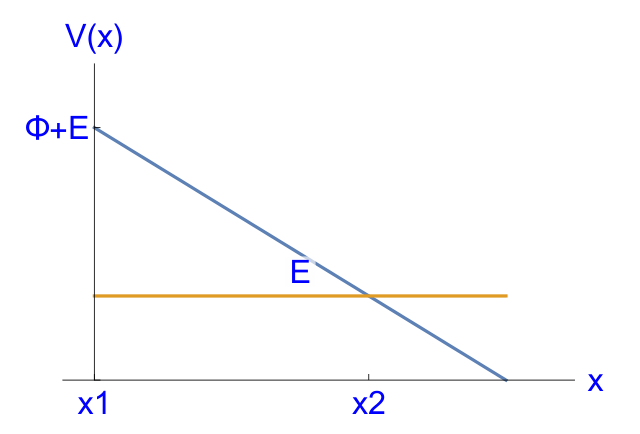
\includegraphics[width=.5\textwidth]{../images/Screenshot 2025-02-17 144752.png}
	\caption{Cold emission potenziale}
	\label{fig:stm}
\end{figure}

\paragraph{STM:}
Il microscopio che sfrutta questo principio, dove la corrente è uguale a:
$$I\propto t(E) \propto \exp(-cd)$$
Quindi per distanze maggiori, la corrente diminuisce esponenzialmente.

\section{Potential well: finita}

Ora immaginiamo che la particella si trova dentro una buca di potenziale FINITA, ovvero che $E < V_0 < \infty$. Vengono fatte delle considerazioni riguardo alla simmetria della buca di potenziale, e che le equazioni sono molto simili allo step a larghezza infinita. Con un discorso sulle probabilità possiamo dire che in pratica che:
$$\rho(x) = \rho(-x)$$
$$|\psi(x)|^2 = |\psi(-x)|^2$$
Le due hanno la stessa probabilità, quindi possono differire al massimo per un fattore di fase.
$$\psi(x) = e^{i\alpha}\psi(-x) \text{ and } \psi(-x) = e^{i\alpha}\psi(x)$$
Quindi sostituendo una versione nell'altra:
$$\psi(x) = e^{2i\alpha}\psi(x)$$
Per mantenere la normalizzazione, $e^{i2\alpha}$ dovrà essere uguale 1 allora viene fuori che $\alpha = 0, \pi$. Questo significa che le soluzioni di $\psi(x)$ possono essere $\pm\psi(-x)$. Questo significa che avremo due diverse classi di soluzioni: \textit{odd} e \textit{even}. Quelle odd saranno del tipo $A\sin(kx)$, mentre le even saranno del tipo $A\sin(kx)$. Questo porterà ad avere lo stesso comportamento ad un estremo (L/2) e il comportamento opposto dall'altra parte (-L/2).

Consideriamo per esempio prima le \textit{even} e imponiamo la continuità di $\psi$ e $\psi'$ 
$$\left\{  \begin{array}{l}
    A\cos(kL/2) = Be^{-gL/2} \\
    -Ak\sin(kL/2) = -Bge^{-gL/2}
\end{array} \right.$$
Possiamo trovare la soluzione di tale problema calcolando la $\tan(kL/2) = g/k$ e introducendo il calcolo dell'energia come una funzione trascendentale:
$$E = \frac{\sqrt{\zeta^2 - (kL/2)^2}}{kL/2}, \text{ dove } \zeta = \sqrt{2mV_0}L/(2\hbar) \text{ e } \zeta \geq kL/2 \geq 0$$
In pratica ci viene data questa energia, che è in funzione di $k$ che ci da un'idea dell'energia della particella e di $L$ che invece si riferisce alla geometria del problema. Quando si plottano queste immagini otteniamo:

\begin{figure}[ht]
	\centering
	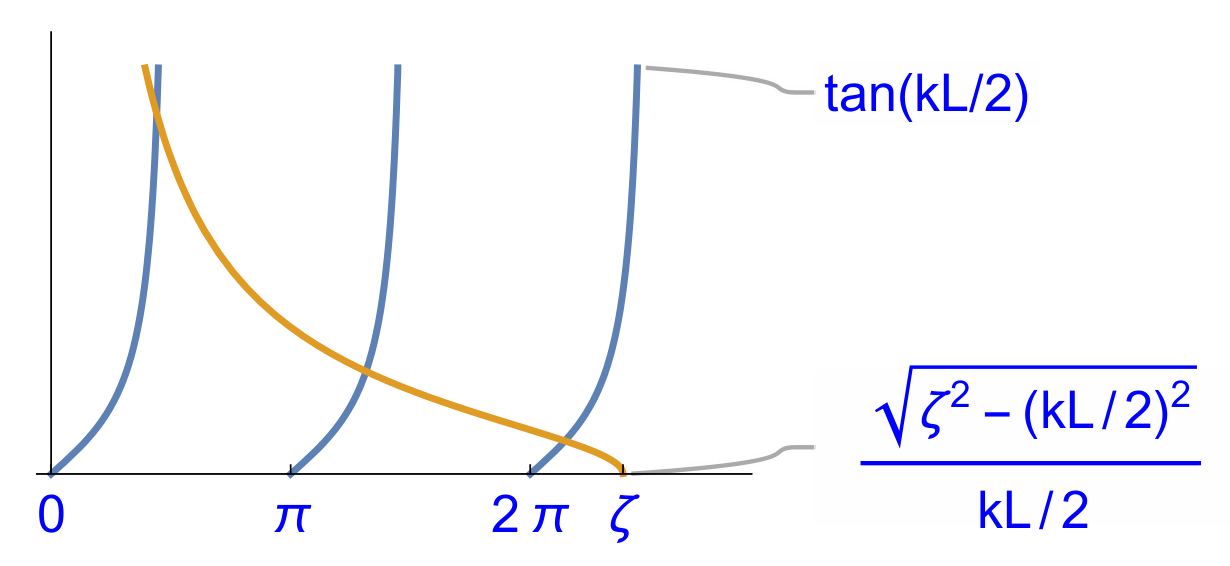
\includegraphics[width=.5\textwidth]{../images/Screenshot 2025-02-17 144454.png}
	\caption{confronto andamento $\psi$ fuori dai limiti}
	\label{fig:zeta_even}
\end{figure}

\noindent Nota come partendo da 0 il plot blu intercetterà sempre almeno un livello di energia, questo è lo stato fondamentale di minor energia possibile. I livelli di energia che possono esistere dentro alla buca di potenziale finita sono limitati. Questo è dovuto anche perchè quando l'energià è maggiore della buca, la particella semplicemente esce.

Risolvendo graficamente possiamo determinare che quindi l'energia del sistema sarà calcolato come:
$$E_n = \frac{\hbar^2k^2_n}{2m} = V_0\frac{(k_nL/2)^2}{\zeta^2}$$ 
Ricorda che il valore di $\zeta$ è dato dalla geometria del problema, in base a questo, possiamo determinare il tipo di energia concessa per quello specifico problema.

Notiamo invece che nel caso invece di onde 'odd' abbiamo un minimo di energia al di sotto dei quali non possono esistere one asimmetriche, che è per $\zeta < \pi/2$.

\section{Potential well: infinita}

Se il potenziale è talmente alto da potersi considerare infinito, allora anche $\zeta \rightarrow \infty$ questo ci porta ad avere l'andamento di $\zeta$ asintotico rispetto alle tangenti, quindi abbiamo virtualmente un'infinito numero di soluzioni, questo inoltre significa che la funziona d'onda decresce così velocemente che possiamo dire che la probabilità di trovare la particella fuori dalla buca di potenziale è 0.

L'unica cosa da sapere è che il valore dell'energia è di:
$$E_n = \frac{\hbar^2k_n^2}{2m} = \frac{[\hbar n\pi]^2}{2mL}, \text{ dove } n = 1, 2, 3, \dots$$ 
Un'altra cosa, la condizione di normalizzazione, ovvero l'ampiezza di A:
$$A=\sqrt{\frac{2}{L}}$$
Questo perchè:
$$1 = |A|^2\int_{0}^{L}dx|\sin(k_nx)|^2 = |A|^2\frac{L}{2} \longrightarrow A=\sqrt{\frac{2}{L}}$$

\section{Parity}

Operatore parità P, cambia la posizione da $x \rightarrow -x$, quindi su una funzione otteniamo:
$$Pf(x) = f(-x)$$
Questo significa che su funzioni even, le lascia invariate, mentre flippa lungo l'asse Y le funzioni odd ($\psi(-x) \rightarrow -\psi(x)$).
Si può inoltre dimostrare che $[P, H] = 0$, questo ci permette quindi di giustificare perchè abbiamo applicato la parità prima senza farci troppi problemi.

\section{$\delta$ holes}

Sono un costrutto matematico in cui abbiamo una potential well infinitamente stretta a profonda, quello che possiamo ricavare è che $\psi(x)$ sarà continua in $x$, mentre la sua derivata sarà discontinua.

Per descrivere questo potenziale usiamo la seguente formula in cui consideriamo il limite per cui $L\rightarrow 0$ e $V_0\rightarrow \infty$ e che il prodotto di $LV_0$ sia costante.
$$V(x) = -V_0L\delta(x)$$
Questo ci permette di separare il problema in 2 parti, dentro al potenziale e fuori, consideriamo prima il fuori:
$$x \neq 0: \frac{d^2\psi(x)}{dx^2}=-\frac{2mE}{\hbar^2}\psi(x)\equiv\kappa^2\psi(x), \text{ dove } \kappa \equiv \sqrt{-2mE}/\hbar$$
Quindi la soluzione generica sarà la somma di due onde (progressiva e regressiva) in una direzione e nell'altra. Ma per evitare che questa diverga, dobbiamo eliminare i due termini 'esplosivi' e successivamente per garantire la continuità, le altre 2 ampiezze dovranno essere uguali. Dunque:
$$\psi(x) = Ae^{-\kappa|x|} = \sqrt{\kappa}e^{-\kappa|x|}$$
Per la parte invece dentro al buco, non voglio risolvere l'integrale, quindi ecco una storiella:
\paragraph{Risoluzione intuitiva:} Dal momento che questa è una buca di potenziale a tutti gli effetti, anche l'andamento di $\zeta$ deve mantenersi uguale. Dato che $\zeta$ varia in funzione di $\sqrt{L}$, allora per $L\rightarrow 0$ anche $\zeta \rightarrow 0$. Se questo è vero, allora $\zeta$ intersecherà solo la prima tangente, quella che passa dallo stato fondamentale, dandoci un solo livello energetico a disposizione. Un'energia più grande permetterebbe di uscire dalla buca.
$$E=-\frac{mV_0^2L^2}{2\hbar^2}$$

\section{Kronig-Penney}

$$V(x) = -LV_0\sum_{n=-\infty}^{\infty}\delta(x-nL)$$
Abbiamo un andamento periodico, ovvero, ogni L di spazio la situazione si ripete. 
Derivazione da spararsi (presenza di potenziali periodici e cambi di variabili, sembra sospettosamente simile a Bloch).
Analizziamo solo il risultato che si ottiene:
$$\cos(\alpha) = \cos(kL) - \frac{mV_0L}{k\hbar^2}\sin(kL)$$
Notiamo che la prima parte è il potenziale periodico, che è simile alla descrizione della funzione di Bloch, dove un certo potenziale riappare nel tempo. La seconda parte invece è più riferita all'attenuazione della funzione d'onda nel tempo, credo sia la conseguenza dell'effetto di riflessione / trasmissione ogni volta che la funzione d'onda incontra un'ostacolo (la buca di potenziale). Più l'energia è grande è più questo termine si riduce, questo suggerisce che a grandi energie la particella si comporta come se il reticolo non esistesse, o come se il reticolo non rappresentasse più un ostacolo per la particella.

\begin{figure}[ht]
	\centering
	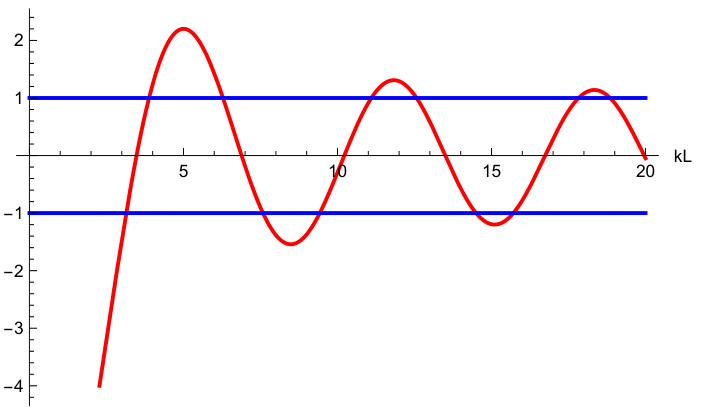
\includegraphics[width=.5\textwidth]{../images/Screenshot 2025-02-17 161537.png}
	\caption{Andamento Kronig-Penney e generazione band-gap}
	\label{fig:kronig}
\end{figure}

\paragraph{Band-Gap:} 
Del grafico rosso, sono solo accettabili le zone in cui la funzione è compresa tra -1 e 1, quindi si formano delle bande accettabili e non. La distanza tra queste bande sono energie che la particella non può assumere all'interno del reticolo, e che quindi viene considerata proibita. Ecco che si generano le band-gap. La natura di conduttore, semiconduttore o isolante dipende da quanto l'ultima banda è riempita: se è piena, il materiale sarà isolante o semiconduttore in base alla dimensione della band-gap, se invece non è piena, sarà un conduttore.


\section{Momento angolare}

\subsection{Introduzione}

Il momento angolare non è altro che:
$$\vec{L} = \vec{x} \wedge \vec{p} $$
Riscritto usando le gli operatori quantistici:
$$\vec{L} \rightarrow -i\hbar\vec{\hat{x}} \wedge \vec{\nabla}$$
Dove ogni singola componente sarà uguale al prodotto vettoriale (caso solo di Z):
$$L_z \rightarrow -i\hbar\left( x\frac{\partial}{\partial y} - y \frac{\partial}{\partial x}\right)$$
Questo quindi ci porta ad ACCETTARE che (ci si basa sulla regola $[\hat{x}_i, \hat{p}_j] = i\hbar\delta_{ij}$):
$$[L_x, L_y] = i\hbar L_z \text{ coordinate sempre ordinate xyz}$$
Scopriamo in generale che invece le componenti del momento angolare commutano con l'operatore posizione e quantità di moto SOLO quando insistono sono sullo stesso asse.
$$[L_z, \hat{z}] = 0$$
$$[L_z, \hat{p}_z] = 0$$
Per proprietà invece che vengono definite sono \textit{Rotationally invariant} ovvero quando non variano di valore al cambiare dell'asse e/o sistema di riferimento, il commutatore farà sempre 0:
$$[L_i, \hat{\vec{p^2}}] = 0$$
$$[L_i, \hat{\vec{x^2}}] = 0$$
$$[L_i, \hat{\vec{L^2}}] = 0$$
Lo possiamo dimostrare, ma non lo faremo :)

\subsection{Eigen-stuff}

Vogliamo sapere quante più cose possibili sul momento angolare, quindi sapendo che per esempio $[L_z, \vec{L}^2] = 0$, possiamo trovare un set base di auto-stati che descrivono il momento angolare, permettendoci di calcolare contemporaneamente sia $L^2$ che $L_z$.

Definiamo quindi un auto-stato $\ket{\beta, m}$ che avrà come autovalori $\beta$ per $\vec{L}^2$ e $m$ per $L_z$:
$$\vec{L}^2 \ket{\beta, m} = \hbar^2\beta\ket{\beta, m}$$
$$L_z \ket{\beta, m} = \hbar m\ket{\beta, m}$$
\textbf{MOLTO IMPORTANTE:} Nota che c'è una grossa differenza, questi $\beta, m$ sono due identificativi di uno stato che sarà un autostato sia di $L^2$ che di $L_z$, possiamo cominciare a calcolare quanto valgono, ma per comodità in futuro otterremo il valore di $\beta$ come funzione di $m$, o meglio, funzione di $m_{max} = l$. Per comodità quindi ci riferiremo all'autovalore di $L^2$ con $l$.
	
\vspace{15pt}

\noindent Il motivo per cui abbiamo aggiunto le diverse $\hbar$ è solo per una questione di analisi dimensionale, dal momento che $\beta$ e $m$ sono semplicemente 2 numeri reali puri.
Dobbiamo inoltre assicurarci che il tutto sia normalizzato, e questo si può imporre:
$$\braket{\beta, m|\beta', m'} = \delta_{\beta\beta'}\delta_{mm'}$$
Ora, noi dobbiamo cercare di definire il meglio possibile questo set base, ed è difficile non usando nient'altro se non gli strumenti che abbiamo a disposizione, per questo introduciamo 2 nuovi operatori. Più avanti scopriremo che si chiamano \textit{Ladder operators}, ma per ora li definiamo solo come una combinazione di componenti X e Y:
$$L_{\pm} \equiv L_x \pm iL_y$$
Questo operatore inoltre, ha la proprietà (il complesso coniugato inverte il valore di $iL_y$):
$$L_{\pm}^{\dagger} = L_{\mp}$$
Le seguenti proprietà vengono rispettate (derivate risolvendo semplicemente il commutatore):
$$[\vec{L}^2, L_{\pm}] = 0$$
$$[L_z, L_{\pm}] = \pm\hbar L_{\pm}$$
$$[L_+, L_-] = 2\hbar L_z$$
Da qui si può inoltre derivare il valore di 2 altre proprietà importanti:
$$L_{\pm}L_{\mp} = L_x^2+L_y^2\pm\hbar L_z$$
$$\vec{L}^2 = L_{\pm}L_{\mp} \mp \hbar L_z + L_z$$
Tutte queste formule sono derivate da combinazioni di equazioni precedenti. 

\vspace{15pt}

\noindent \textbf{Nelle future equazioni se trovi il simbolo $\circledcirc \_ \circledcirc$, significa che il passaggio è stato compiuto usando una di queste formule dei commutatori.}

\newpage

\subsection{Ladder operator}

\begin{figure}[ht]
	\centering
	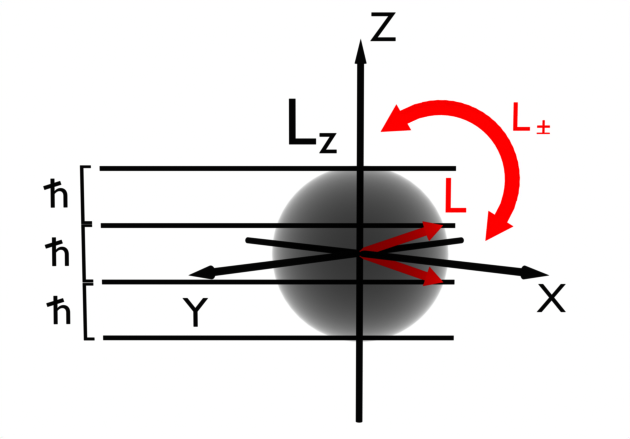
\includegraphics[width=.5\textwidth]{../images/ladder.png} 
	\caption{Spiegazione geometrica del ladder operator}
	\label{fig:ladder}
\end{figure}

\noindent Possiamo interpreatare il ladder operator come la rotazione del momento angolare lungo una delle direzioni generiche composte da X e Y (non ci interessa molto la direzione precisa, dal momento che a causa del principio di indeterminazione sappiamo solo che questa rotazione sarà uguale ad un shift di energia pari a $\hbar$.

Questo ci permette di ottenere $L_z$ in tutte le possibili suddivisioni dell'energia in $\Delta E = \hbar$. Ecco perchè all'aumentare dell'energia aumenteranno i possibili $m$ e perchè quando $l$ e $m$ coincidono abbiamo il massimo valore di $L_z$: $L_z$ e $L$ coincidono come direzione.

Il motivo per cui ci possiamo spostare solo di intervalli di $\hbar$ è dovuto al fatto che i commutatori ci dicono così. Un modo più intuitivo di vederlo è immaginarsi di avere un vettore in 3D le cui componenti possono essere SOLO dei numeri interi. Se vogliamo aumentare o diminuire di 1 il valore della componente Z dovremo adeguare di conseguenza X e Y. Questo lo possiamo fare a patto che seguiamo 2 regole: Tutte le variazioni devono essere numeri interi e il modulo totale del vettore deve rimanere invariato.

\subsection{Derivazione di $\beta$ e $m$}
Possiamo inanzitutto trovare una relazione tra questi 2 autovalori notando che da questa espressione abbiamo:
$$\braket{\beta, m | \vec{L}^2 | \beta, m} = \braket{\beta, m | L_x^2 | \beta, m} + \braket{\beta, m | L_y^2 | \beta, m} + \braket{\beta, m | L_z^2 | \beta, m} $$
Sappiamo che $L^2 \propto \hbar^2 \beta$, mentre $L_z^2 \propto \hbar^2 m^2$. Se consideriamo che che sia $L^2_x$ che $L^2_y$ saranno $\geq 0$, otteniamo la seguente relazione tra gli autovalori di {$\beta$} e {$m$}:
$$\beta \geq m^2 \geq 0$$
Questo significa che questo $m$ sarà limitato ad essere compreso tra 2 valori:
$$m_{min} = k, \text{ } m_{max} = l$$
Ora che abbiamo introdotto il ladder operator, proviamo ad applicarlo al sistema per scoprire come agiscono, quanto valgono e se il sistema rimane un autostato di $\vec{L}^2$ e di $L_z$:

\begin{itemize}
	\item $\vec{L}^2$, prima di tutto scambiamo l'ordine (tanto commutano). Poi, sappiamo quanto vale l'autovalore di $\vec{L}^2 \rightarrow \hbar^2\beta$ $\circledcirc \_ \circledcirc$, quindi scambiando l'ordine abbiamo la possibilità di applicare subito $\vec{L}^2$ e in questo modo avere il ket moltiplicato solo per il ladder operator.
	$$\vec{L}^2 (L_+\ket{\beta, m}) = L_+\vec{L^2} \ket{\beta, m} = \hbar^2 \beta (L_+\ket{\beta, m})$$
	Questo ci dà informazioni sul fatto che l'operatore agendo lascia l'autostato in un autostato e che ha autovalore pari a $\hbar ^ 2\beta$.
	\item $L_z$, vogliamo fare la stessa cosa, ma $[L_z, L_{\pm}] = \pm \hbar L_{\pm}$, quindi il risultato sarà:
	$$L_z(L_+\ket{\beta, m})$$
	$$([L_z, L_+] + L_+L_z)\ket{\beta, m}$$
	$$\hbar L_+\ket{\beta, m} + L_+(L_z\ket{\beta, m})$$
	$$\hbar L_+\ket{\beta, m} + L_+\hbar m \ket{\beta, m}$$
	$$\hbar L_+ (m+1) \ket{\beta, m} \rightarrow L_+\ket{\beta, m} \propto \ket{\beta, m + 1}$$
\end{itemize}

\noindent Abbiamo constatato che l'operatore ladder aumenta o diminuisce di 1 l'autovalore $m$ restituendoci ancora un autostato dell'operatore $L^2$ o $L_z$. Il fatto che possa anche diminuire viene fuori dai calcoli, qual'ora sostituissi il commutatore con il meno.

Deriviamo inoltre un'importante limitazione: dato che $m$ non può essere $> l$, allora quando $m = l$:
$$L_+\ket{\beta, l} = 0$$
Un'altra considerazione da fare è che quando applichiamo $L_-$ dopo aver applicato $L_+$ allo stato più alto possibile $\ket{\beta, l}$ dovrà restuire 0 (piccola nota, qui non abbiamo usato direttamente la conseguenza del commutatore $\circledcirc \_ \circledcirc$, invece abbiamo sostituito $L^2_x + L^2_y$ con $L^2 - L^2_z$):
$$0 = L_-L_+\ket{\beta, l} = (\vec{L}^2 -\hbar L_z -L^2_z)\ket{\beta, l}$$
Conoscendo però gli autovalori corrispondenti ad $L^2$ e $L_z$ otteniamo:
$$\hbar^2 (\beta - l - l^2) \ket{\beta, l}$$
Scoprendo quindi che la relazione che c'è tra $\beta$ e $m$ è:
$$\beta = l(l+1) \text{, dove } l = m_{max}$$
Facendo la stessa identica cosa, ma sull'estremo inferiore otteniamo la stessa relazione ma con $k = m_{min}$:
$$\beta = k(k-1)\text{, dove } k=m_{min}$$
Comparando i risultati è chiaro che  $k = -l$. Inoltre, sapendo che i ladder operator modificano di 1 gli autovalori ogni volta che agiscono, sappiamo che tutti i valori di $m$ saranno \textit{integer-spaced}, nel range che va da $[-l, l]$. Per sottostare a questa limitazione, allora $l$ dovrà essere un \textit{semi-integer}.

\vspace{15pt}

\noindent Se può servire, data una certa $l$, il numero di $m$ a tua disposizione seguirà la formula: $2l + 1$

\vspace{15pt}

\noindent Sapendo ora scrivere l'autovalore di $L_2$ in funzione del valore massimo che può esprimere l'autovalore di $L_z$, riscriveremo d'ora in avanti gli autostati in funzione di 2 nuovi termini:
$$\vec{L}^2\ket{l, m} = \hbar^2 l(l+1)\ket{l, m}$$
$$L_z\ket{l, m} = \hbar m\ket{l, m}$$

\paragraph{Normalizzazione:}
Un'ultima cosa che possiamo fare è calcolare il fattore di normalizzazione ogni volta che applichiamo il ladder operator, di fatto ci viene chiesto di calcolare $\braket{l, m | L^{\dagger}_{\pm}L_{pm}|l, m}$ che corrisponde a calcolare il $[L_+, L_-]$, ovvero il risultato del calcolo di $\beta$ con il valore massimo e il valore minimo:
$$|C_{\pm}|^2 = \hbar^2[l(l+1) - m(m\pm 1)]$$
Ottenendo il valore solo per $C_{\pm}$ uno ottiene che:
$$L_{\pm}\ket{l, m} = \hbar\sqrt{l(l+1) - m(m\pm 1)}\ket{l, m\pm1}$$

\subsection{Coordinate sferiche}

Inanzitutto vediamo come le vecchie coordinate si trasformano in quelle nuove:


\begin{minipage}{0.45\textwidth} % Larghezza prima colonna
    \centering
    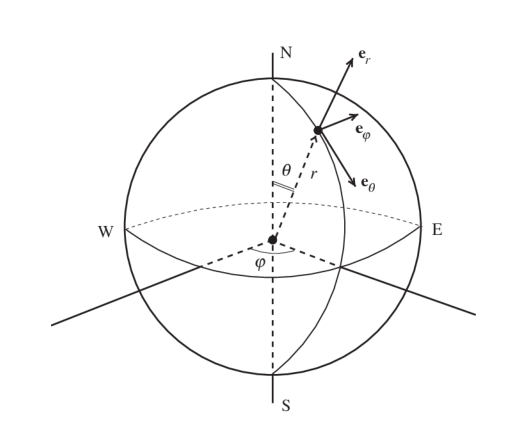
\includegraphics[width=0.9\textwidth]{../images/Screenshot 2025-02-18 175342.png} 
    \captionof{figure}{Sistema di riferimento polare}
    \label{fig:polar}
\end{minipage}
\hfill % Separazione tra le due colonne
\begin{minipage}{0.45\textwidth} % Larghezza seconda colonna
    Posizione:
	$$\left\{ \begin{array}{l}
		x = r \sin(\theta)\cos(\varphi)\\
		y = r \sin(\theta)\sin(\varphi)\\
		z = r \cos(\theta)
    \end{array} \right.$$
	\vspace{15pt}
	
	\noindent Derivata della posizione:
	$$\nabla = \vec{e}_r \frac{\partial}{\partial r} + \vec{e}_{\theta} \frac{1}{r}\frac{\partial}{\partial \theta} + \vec{e}_{\varphi} \frac{1}{r\sin(\theta)}\frac{\partial}{\partial \varphi}\\$$
\end{minipage}

\vspace{15pt}

\noindent È utile definire un set di versori che rappresentano la direzione in cui le grandezze $\theta$, $\varphi$ e $r$ cambiano nel tempo. Ora sono combinazioni di seni e coseni. Se vuoi ripeterli li trovi a pagina 45 delle note. Per ora troviamo solo la soluzione alla conversione di $L_z$ in coordinate polari. 
$$\bra{\theta, \varphi}L_z = \bra{\theta, \varphi}\vec{e}_z\vec{L} = -i\hbar \frac{\partial}{\partial \varphi} \bra{\theta, \varphi}$$
Come possiamo notare, il risultato è l'applicazione della derivata alla coordinata Z in coordinate polari. Si può fare la stessa cosa per $L^2$, ma diventi scemo, quindi: RICORDA:
$$\bra{\theta, \varphi}\vec{L}^2 = -\hbar^2 \left[\frac{1}{\sin(\theta)} \frac{\partial}{\partial \theta}\left(\sin(\theta) \frac{\partial}{\partial \theta}\right) + \frac{1}{\sin^2(\theta)} \frac{\partial^2}{\partial^2\varphi}\right]\bra{\theta, \varphi}$$
\paragraph{Armoniche sferiche:}
Si può rappresentare l'autostato $\ket{l, m}$ come funzioni $Y_{lm}(\theta, \varphi)$ in coordinate sferiche:
$$\braket{\theta, \varphi | l, m} \equiv Y_{lm}(\theta, \phi) = \Theta(\theta)\Phi(\varphi)$$
Nota come il risultato è un prodotto di funzioni, una solo in funzione di $\theta$, e l'altro solo in funzione di $\varphi$.

\paragraph{Calcolo dei polinomi:} 
Bene, abbiamo calcolato quanto valgono gli operatori in coordinate polari, sappiamo anche che l'autostato $\ket{l, m}$ si può rappresentare come $Y_{lm}$. Calcoliamo allora quanto valgono queste funzioni $Y_{lm}$ per i diversi autostati conoscendo il valore degli operatori.
$$\braket{\theta, \varphi | L_z | l, m} = (\bra{\theta, \varphi}L_z)\ket{l, m} = \bra{\theta, \varphi}(L_z \ket{l, m})$$
Dai calcoli prima abbiamo che:
$$-i\hbar\frac{\partial}{\partial \varphi} \braket{\theta, \varphi|l, m} = \hbar m \braket{\theta, \varphi | l, m}$$
Sostituendo con $Y_{lm}$ possiamo semplificare $\Theta(\theta)$ dal momento che non abbiamo nulla in funzione di $\theta$.
$$-i\hbar\frac{\partial}{\partial \varphi} \cancel{\Theta(\theta)}\Phi(\varphi) = \hbar m \cancel{\Theta(\theta)}\Phi(\varphi)$$
Quello che rimane è solo un'equazione differenziale, la cui soluzione è:
$$\Phi(\varphi) = e^{im\varphi}$$
BTW, per il futuro possiamo già calcolarci la derivata seconda e scoprire che la soluzione non è altro che la funzione stessa moltiplicata per un fattore:
$$\frac{\partial^2 \Phi(\varphi)}{\partial \varphi^2} = -m^2\Phi (\varphi)$$
Possiamo fare la stessa cosa, ma sostituendo le varie componenti di $L^2$ e non di $L_z$.
Casino assurdo, la formula è mastodontica. Quello di buono che c'è da sapere è che da tutto quel casino possiamo estrarre il termini in $\Phi(\varphi)$ dal momento che sappiamo calcolare la sua derivata seconda, e non solo: possiamo semplificare il tutto rendendo l'equazione una sola funzione di $\Theta(\theta)$.

\paragraph{Polinomi di Legendre:}
Una cosa carina che ci viene detta più avanti è che 
$$\Theta(\theta) = P^m_l\cos(\theta)$$
Quindi abbiamo tutto per descrivere $Y_{lm}$:
$$Y_{lm}(\theta, \varphi) = \Theta(\theta)\Phi(\varphi) \propto P^m_l\cos(\theta)e^{im\varphi}$$
Esiste un fattore di normalizzazione che si ricava risolvendo sta bestia: SKIP.

\paragraph{Parità: importante esame}
Con la parità puoi calcolare i vari valori che ti vengono chiesti all'esame: 
$$PY_{lm}(\theta, \varphi) = Y_{lm}(\pi - \theta, \pi + \varphi) = e^{im\pi}(-1)^{l+|m|} Y_{lm}(\theta, \varphi) = (-1)^lY_{lm}(\theta, \varphi)$$
Actually, il modo per non sbagliare mai è seguire le seguenti regole (proprietà intellettuale di Cimma \& Capellino\texttrademark):
\begin{itemize}
	\item Se un termine dell'equazione ha dipendenza solo da $r$ allora $l=0, m=0$.
	\item Se un termine non ha dipendenza di $\theta$ allora $l=0$.
	\item Se un termine non ha dipendenza di $\varphi$ allora $m=0$.
	\item Guarda ogni termine dell'equazione e calcola quanto vale il grado più alto del termine $\theta$ e $\varphi$, questo corrisponderà ad $l$ e $m$ rispettivamente.
	$$\cos(\theta)\sin^2(\varphi) + \sin(\varphi) \rightarrow l=1, m=\pm2, \pm1$$
	\item Se il termine con $\phi$ è un esponenziale complesso e non un seno, il termine di $m$ sarà solo del segno dell'esponente, sarà invece $\pm$ nel caso di un seno.
	\item Nel caso tu abbia $\cos^2(\theta)$, $l$ varrà non solo 2 ma anche 0. Questo è dovuto a com'è scritta l'armonica in questo caso: ha anche un termine senza dipendenza da $\theta$.
\end{itemize}

\noindent Questo copre tutte le casistiche fino ad $l, m = 2, \pm2$.

\section{Spin}

\subsection{Stern-Gerlach}

RICORDA: Quando dicono che lo strumento è allineato \textit{Along 'x' axis} significa che il CAMPO MAGNETICO è allineato lungo quell'asse, non lo strumento!

\vspace{15pt}

\noindent Cominciamo con l'introdurre che il campo magnetico esercita su particelle cariche come gli elettroni una forza pari a:
$$F_z = -\frac{\partial}{\partial z}\left(-\vec{\mu}\cdot\vec{B}\right) = \mu_z\frac{\partial B(z)}{\partial z}$$
$$\mu_z = \frac{e}{2m_e}L_z$$
This way we can relate the $F_z \propto L_z$.

\paragraph{Preambulo:}
Se consideriamo un fascio di elementi con momento angolare 0, notiamo comunque uno splitting del raggio, questo ci suggerisce la presenza di un altro momento angolare legato a qualche altra caratteristica della particella: spin elettrone. Possiamo assumere che si comporta esattamente come il momento angolare classico, e quindi, varranno le seguenti proprietà (consideriamo $s$ con il valore più piccolo possibile $\frac{1}{2}$):
$$\vec{S}^2 \rightarrow \hbar^2s(s+1) \rightarrow \frac{3}{4}\hbar^2$$
$$S_z \rightarrow \pm \frac{\hbar}{2}$$

\paragraph{Caso di apparati in successione:}

Avviene un fenomeno interessante, se isoliamo il fascio allineato lungo $z_+$ e lo facciamo viaggiare attraverso un allineatore lungo x e di nuovo selezioniamo solo la direzione $x_+$ scopriremo con divertito stupore che facendolo ripassare in un allineatore z, si formeranno entrambi i raggi: $z_+, z_-$.
È come se una volta che passano in un magnete orientato diversamente si allineassero lungo quell'asse, ma ogni spin con direzione diversa. Il motivo per cui sono presenti entrambi gli spin, è perchè la direzione iniziale era perpendicolare, quindi per cambiare di nuovo asse hanno il $50\%$ di probabilità di capitare girati in sù o in giù.

\begin{figure}[ht]
	\centering
	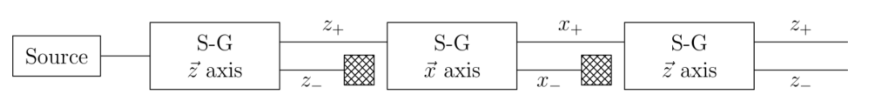
\includegraphics[width=1\textwidth]{../images/Screenshot 2025-02-19 125717.png} 
	\caption{Stern - Gerlach apparati in successione}
	\label{fig:stern}
\end{figure}

\subsection{Teoria}

Dato che abbiamo capito che possono esistere al massimo due stati diversi, per comodità li rappresenteremo come:
$$\left| \frac{1}{2}, \frac{1}{2} \right> \equiv \ket{+}$$
$$\left| \frac{1}{2}, -\frac{1}{2} \right> \equiv \ket{-}$$
Questo significa che per rappresentare TUTTI i possibili autostati legati allo spin possiamo usare:
$$\ket{\pm} \rightarrow \vec{S}^2 \ket{\pm} = \hbar^2\frac{3}{4}\ket{\pm} \rightarrow \vec{S}_z \ket{\pm} = \pm \hbar \frac{1}{2} \ket{\pm}$$

\paragraph{Commutatori \& Ladder:}
Stesse identiche formule, semplicemente il range di l e m sono ridotti notevolemente e cambiano nome in s e $m_s$.

\paragraph{Matrici di Pauli:}
Dal momento che possiamo avere solo due situazioni, in cui abbiamo o lo stato + o lo stato -, possiamo rappresentare più facilmente e comodamente tutti i calcoli con vettori e matrici:
$$\ket{+} \equiv \left(\begin{array}{c}
	1 \\
	0 \\
\end{array}\right) \text{ and }
\ket{-} \equiv \left(\begin{array}{c}
	0 \\
	1 \\
\end{array}\right)$$
Questo ci viene molto comodo, dal momento che possiamo rappresentare tutti i possibili stati in maniera estremamente compatta: Rappresentiamo gli operatori lungo le varie direzioni $xyz$ andando semplicemente a calcolare l'effetto che provoca l'applicazione dell'operatore su un autostato e riportando il suo autovalore. Di fatto quello che abbiamo fatto è stato creare una 'look-up table' che ci permette di trovare il giusto autovaloro dato un autostato e la matrice dell'operatore associata.

Possiamo inoltre interpretare ogni colonna come l'autostato in cui finirà uno spin dopo aver applicato l'operatore considerato (prima colonna spin +, seconda colonna spin -).
Riscrivendo le matrici di Pauli (ricorda, c'è sempre un fattore moltiplicativo di $\frac{\hbar}{2}$):
$$\sigma_x = \left(\begin{array}{lr}
	0 & 1\\	
	1 & 0\\	
\end{array}\right),
\sigma_y = \left(\begin{array}{lr}
	0 & -i\\	
	i & 0\\	
\end{array}\right),
\sigma_z = \left(\begin{array}{lr}
	1 & 0\\	
	0 & -1\\	
\end{array}\right),$$
Quindi, ora sappiamo cosa succede ad uno spin quando lo misuriamo lungo un asse diverso dal suo originario. La misura stessa però introduce nel sistema dell'eenrgia / perturbazione, (chiamala come vuoi) che andrà a destabilizzare il sistema al punto che la probabilità di trovare la particella orientata in una direzione o l'altra si è completamente resettata.

Qualunque stato di spin può essere scritto come combinazione lineare di stati $\ket{+}$ e $\ket{-}$. Quanto più lo spin "assomiglierà" come direzionalità ad un asse, più sarà probabile che mantenga il suo stato di spin.

\subsection{Gyromagnetic factor / MRI}
Di importante c'è da dire che il fattore giromagnetico è determinato dalla somma degli effetti del momento magnetico orbitale e di quello di spin:
$$\mu = \mu_{orbit} + \mu_{spin}$$
$$\mu = \frac{e}{2m_e} (L + 2S), \text{ dove } 2 = g$$
$$S = \frac{\hbar}{2}\sigma \rightarrow \mu_{tot} = -\frac{|e|\hbar}{2m_e}\left(\frac{L}{\hbar}+\sigma\right)$$
Se ti ricordi the \textit{Bohr magneton}, meglio:
$$\mu_B = \frac{|e|\hbar}{2m_e}$$

\paragraph{MRI cose importanti:} Quando inserisci uno spin lungo una generica direzione $n$ dentro ad un campo magnetico orientato lungo un asse, lo spin comincierà a girare attorno a quell'asse. Ora, se calcoli S lungo lo stesso asse, non ti cambia nulla, avrai solo lo spin che gira, ma la misura di per se non cambia. D'altro canto, se misuri lungo un altro asse allora si avrà una componente che cambia nel tempo modificando le probabilità di trovare spin up o down. Ecco la formula per ricavare questa frequenza chiamata \textit{Larmor Frequency}:
$$\omega_L = \frac{g|e|B_0}{2m}$$

\section{Somma di 2 spin}

Quello che vogliamo fare ora è vedere se riusciamo a calcolare come 2 spin si sommano tra loro (intereagiscono) e vedere quante più cosa possiamo sapere contemporaneamente su di essi.
Per iniziare possiamo dire che per un sistema di 2 elettroni avremo che il generico stato di spin sarà la combinazione lineare di:
$$\ket{s_1,m_{s1};s_2,m_{s2}} = \left\{\ket{++}, \ket{+-}, \ket{-+}, \ket{--}\right\}$$
Dove 1 è riferito al primo elettrone, mentre 2 al secondo. Il problema è che questo base non descrive efficientemente questo stato. Il problema è dovuto al fatto che $\vec{S}^2$ commuta con $S_z = S_{1z} + S_{2z}$, ma non con i singoli termi individualmente. Questo significa che se il sistema si trova in uno degli stati sopra elencati, potremmo non conoscere lo spin totale, dal momento che questi stati individualmente non sono autostati di $\vec{S}^2$ (solo la loro combinazione è un autostato).

Ecco perchè ripartiamo per l'ennesima volta dalla formula:
$$\vec{S}^2 \ket{S, M} = \hbar^2S(S+1)\ket{S, M}, \text{ e } S_z\ket{S,M} = \hbar M\ket{S,M}$$
Applicando quindi l'operatore $S_z$ per esempio ai diversi stati vediamo che:
$$\begin{array}{l}
	S_z\ket{++} = (S_{1z} \ket{+}) \ket{+} + \ket{+} (S_{2z}\ket{+}) = \hbar\ket{++}\\\\
	S_z\ket{--} = (S_{1z} \ket{-}) \ket{-} + \ket{-} (S_{2z}\ket{-}) = -\hbar\ket{++}\\\\
	S_z\ket{+-} = (S_{1z} \ket{+}) \ket{-} + \ket{+} (S_{2z}\ket{-}) = 0\\\\
	S_z\ket{-+} = (S_{1z} \ket{-}) \ket{+} + \ket{-} (S_{2z}\ket{+}) = 0\\\\
\end{array}$$
Per spiegare cosa succede, ricorda che ogni operatore agisce solo sulla sua componente (1 solo su 1 e 2 solo su 2), quindi dato che $S_z = S_{1z} + S_{2z}$ abbiamo questo risultato. Gli 0 li otteniamo perchè otteniamo esattamente lo stesso risultato ma di segno opposto, di fatto annullandosi.	

Applicando le stesse identiche formule, possiamo anche calcolare quanto vale $L_2$, lo farò? No.
L'unica cosa effettivamente importante è che da tutti questi calcoli viene fuori che l'autovalore sono 1 nel caso di $\ket{++}$ e -1 per $\ket{--}$ ($\vec{S}^2 \ket{++} = 2\hbar^2\ket{++}$). Questo ci dice che il valore massimo (S) sarà 1, mentre (M) varierà tra -1 e 1. 
Sapendo perà che il numero di $M$ che dovremmo trovare è $= 2S + 1 = 3$, applichiamo il ladder operator ottenendo lo stato $\ket{1,0}$. Noi però siamo partiti con 4 equazioni, ma abbiamo solo 3 soluzioni per ora. Dobbiamo trovare un altro stato ancora ortonormale ai primi 2: invertendo 
$$\ket{1, 0} = \frac{1}{\sqrt{2}}\left(\ket{+-} + \ket{-+}\right)$$
Otteniamo:
$$\ket{0, 0} = \frac{1}{\sqrt{2}}\left(\ket{+-} - \ket{-+}\right)$$
Questi identificano le varie combinazioni che noi conosciamo come singoletto, doppietto e tripletto.

\section{Somma di spin con momento angolare}

Ora invece proviamo a calcolare il momento angolare tot. dello spin sommando lo spin dell'elettrone con il momento angolare dell'orbitale:
$$\vec{J} = \vec{S} + \vec{L}$$
Questo ci porta ad avere un autostato bestiale:
$$\ket{l,m;s,m_s} = \left\{\ket{l,m;\frac{1}{2},\frac{1}{2}}, \ket{l,m;\frac{1}{2},-\frac{1}{2}}\right\} = \left\{\ket{l,m,+}, \ket{l, m, -}\right\}$$
Dato che abbiamo dei problemi a quanto pare, RICALCOLIAMO PER LA 4° VOLTA LA STESSA IDENTICA COSA PER $J^2$ E $J_z$ YIPPIE:
$$\vec{J}^2 = (\vec{S}^2 + \vec{L}^2)$$
$$J_z = S_z + L_z$$
$$\ket{J, M}$$
Come al solito partiamo con il calcolare $J_z$ e $\vec{J}^2$ partendo dallo stato più alto possibile:
$$J_z\ket{l,l,+} = \left(L_z \ket{l,l}\right)\ket{+} + \ket{l,l}(S_z\ket{+})=\hbar\left(l+\frac{1}{2}\ket{l,l,+}\right)$$
Questo risultato è dato dal fatto che ogni operatore opera solo sulla sua parte, il risultato è la somma di tutto, abbiamo quindi che $L_z$ ci dà come risultato $\hbar l$, mentre $S_z$ dà $\frac{\hbar}{2}$.
Nel caso di $\vec{J}^2$ è leggermente più complesso (la parte con gli operatori è la trasformazione da $L = L_x + L_y + L_z$ in $L_z + L_{\pm}$):
$$\vec{J}^2\ket{l,l,+} = \left(\vec{L}^2 + \vec{S}^2 + {2L_zS_z + L_-S_+ + L_+S_-}\right)\ket{l,l,+}$$
Ora, fortunatamente questi termini con il ladder vanno a 0, perchè per entrambi gli operatori siamo in un estremo :)

Applicando invece gli operatori rimasti, abbiamo una parte uguale al risultato di $J_z$, più l'altra derivante dai termini quadri:
$$\vec{J}^2 = \hbar^2(l+1/2)(l+3/2)\ket{l,l,+}$$
Risolvendo per $l$ otteniamo che gli autovalori $J$ e $L$ sono entrambi $l + 1/2$. Per ottenere gli altri possibili stati applichiamo il ladder operator a manetta finchè non esauriamo tutte le soluzioni.
$$J_-\ket{l,l,+} = \ket{l,l}\left(S_-\ket{+}\right) + \left(L_-\ket{l,l}\right)\ket{+} = \hbar\ket{l,l,-} + \hbar\sqrt{l(l+1) - l(l-1)  \ket{l,l-1,+}}$$
Basta, il resto non è importante. Puoi continuare ad applicare il ladder operator.

\section{Perturbation theory (NON - DEGENERATE)}

Equazione principale di questo capitolo:
$$H = H_0 + \lambda H_1, \text{ con } \lambda \ll 1$$
Partiamo dal fatto che l'Hamiltoniana non perturbata è definita come:
$$H_0\ket{n^{(0)}} = E_n^{(0)}\ket{n^{(0)}}, \text{ dove } \braket{n^{(0)}|m^{(0)}} = \delta_{mn}$$
Noi vogliamo trovare gli \textit{energy levels} e funzioni d'onda che soddisfino:
$$H\ket{n} = E_n\ket{n}, \text{ dove } \braket{n|m} = \delta_{mn}$$
\paragraph{Come facciamo? Espansione:}
$$
\begin{array}{l}
	\mathcal{O}(\lambda^0): H_0\ket{n^{(0)}} = E_n^{(0)}\ket{n^{(0)}}\\
	\mathcal{O}(\lambda^1): H_0\ket{n^{(1)}} + H_1\ket{n^{(0)}} = E_n^{(0)}\ket{n^{(1)}} + E_n^{(1)}\ket{n^{(0)}}
\end{array}
$$
Il motivo per cui l'espansione procede in questo modo è perchè i termini più "importanti" ovvero $H_0$ agisce sul grado più alto considerato, mentre la perturbazione agisce sullo stato già calcolato di livello più basso: quello che succede è applicare la piccola perturbazione sullo stato già conosciuto e applicare l'hamiltoniana base conosciuta sul nuovo stato che quindi ora avrà anche il nuovo contributo.
$$\braket{n^{(0)}|H_0|n^{(1)}} + \braket{n^{(0)}|H_1|n^{(0)}} = \braket{n^{(0)}|E_n^{(0)}|n^{(1)}} + \braket{n^{(0)}|E_n^{(1)}|n^{(0)}}$$
$$\cancel{E_n^{(0)}\braket{n^{(0)}|n^{(1)}}} + \braket{n^{(0)}|H_1|n^{(0)}} = \cancel{E_n^{(0)}\braket{n^{(0)}|n^{(1)}}} + E_n^{(1)} \braket{n^{(0)}|n^{(0)}}$$
Otteniamo quindi in questo modo l'energia associata alla perturbazione:
$$E_n^{(1)} = \braket{n^{(0)}|H_1|n^{(0)}}$$
\paragraph{IMPORTANTE:} Ricorda che puoi riscrivere sempre lo stato $\ket{n^{(1)}}$ come combinazione lineare:
$$\ket{n^{(1)}} = \sum_{j \neq n} c_{nj}\ket{j^{(0)}}$$
Esiste una dimostrazione (pagina 63) che ci permette di calcolare $c_{nl}$ in funzione dei dati in nostro possesso:
$$c_{nl} = \frac{\braket{l^{(0)}|H_1|n^{(0)}}}{E_n^{(0)}-E_l^{(0)}}$$
Quindi ora possiamo riscrivere l'autostato come:
$$\ket{n^{(0)}} = \sum_{j \neq n} \frac{\braket{l^{(0)}|H_1|n^{(0)}}}{E_n^{(0)}-E_l^{(0)}} \ket{j^{(0)}}$$
TADA, l'unico motivo per cui questo è considerato un caso non degenere è perchè assumiamo che il denominatore è $\neq 0$, ovvero $E_n^{(0)} \neq E_l^{(0)}$, il caso degenere invece considera il caso in cui i due termini siano uguali.

\section{Zeeman normale}
Quando avevamo parlato del Gyromagnetic factor, avevamo accennato a quanto valesse l'effetto del momento magnetico nell'elettrone. Ora vediamo che questo effetto torna qui per descrivere come viene pertrubato il sistema:
$$H = \underbrace{-\frac{\hbar^2 \nabla^2}{2m_e} - \frac{e^2}{4\pi\epsilon_0 r}}_{\equiv H_0} + \frac{\mu_B}{\hbar} B L_z$$
Questo contributo lo possiamo considerare molto piccolo nel caso di campi magnetici estremamente piccoli. Quello che succede è che abbiamo uno splitting dei livelli energetici in base alla $l$ dell'orbitale preso in considerazione:

\begin{figure}[ht]
	\centering
	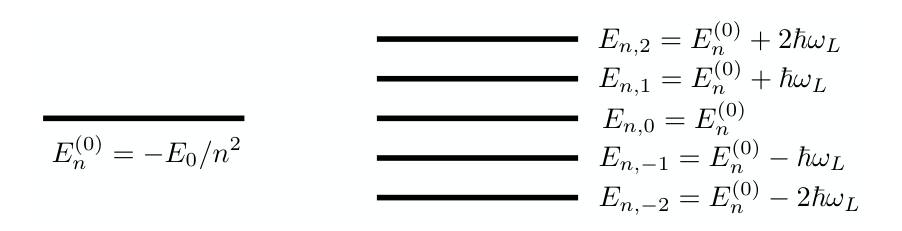
\includegraphics[width=1\textwidth]{../images/Screenshot 2025-02-21 165431.png}
	\caption{Zeeman effect: level splitting}
	\label{fig:zeeman_normal}
\end{figure}

Io me spiego che la presenza delle varie suddivisioni è legata alla quantità di energia intrinseca presente dentro all'orbitale: più energia è presente e più questa può suddividersi e generare livelli diversi (degeneri).

La spaziatura dei livelli energitici qui è costante, dato che l'unica dipendenza che c'è è quella legata ad $l$, ed $l$ ha intervalli regolari. Per conoscere il valore dell'energia, usa la formula:
$$E_{n,m} = -\frac{E_0}{n^2}+ \hbar\omega_Lm$$
$$\Delta E = \hbar\omega_L$$

\section{Relativistic correction}

Questa si basa sul considerare che l'elettrone si muove a velocità estremamente elevate, al punto da subire l'effetto relativistico del suo movimento. Ecco che alla Hamiltoniana aggiungiamo l'energia relativa:
$$E = \sqrt{\vec{p}^2c^2 + m_e^2c^4} = \underbrace{m_ec^2 + \frac{\vec{p}^2}{2m_e}}_{H_0} \underbrace{- \frac{1}{8}\frac{(\vec{p^2})^2}{m_e^3c^2}}_{H_1} + ...$$
Puoi quindi fare il calcolo per ottenere il valore del nuovo stato:
$$\braket{n,l,m|H_1|n,l,m}$$

\section{Interazione: Spin - orbita}
Imma be honest, non ho capito 'na mazza...

\section{Zeeman anomalous}
Somma di tutti gli effetti visti fino ad ora, modificano l'effetto Zeeman, andando ad ottenere delle suddivisioni più ricche:

\begin{figure}[ht]
	\centering
	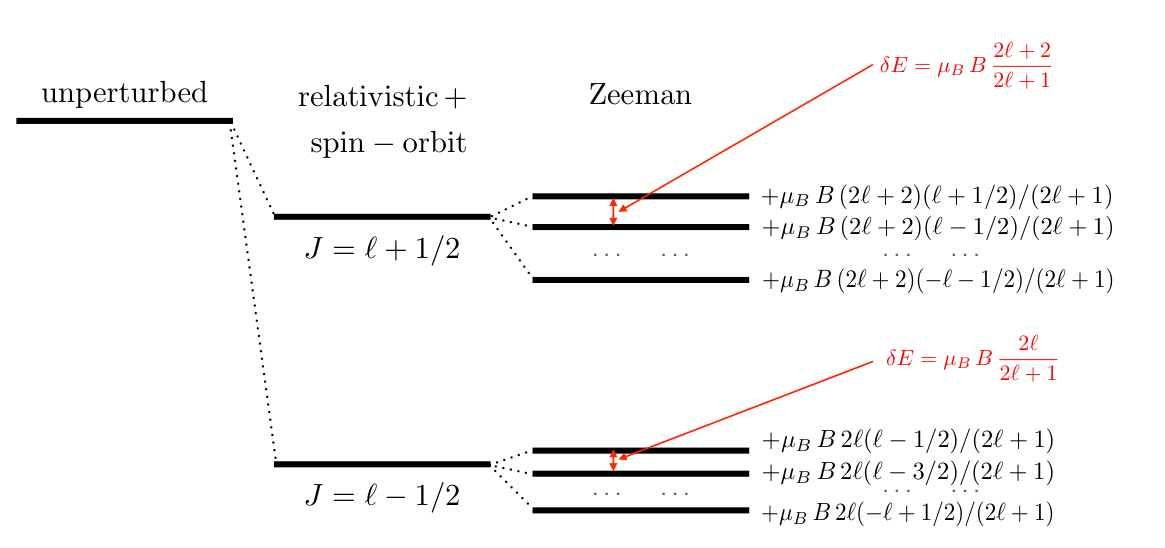
\includegraphics[width=1\textwidth]{../images/Screenshot 2025-02-21 192037.png}
	\caption{Anomalous Zeeman}
	\label{fig:anomalous_zeeman}
\end{figure}

L'importante è notare come le suddivisioni tra i livelli non sono costanti:
\begin{itemize}
	\item per $l+1/2$ abbiamo una distanza maggiore, dovuta da una somma costruttiva di termini (nell'anomalous ci sono termini dipendenti dai numeri quantici e altri no). Se tutti i termini sono costruttivi ci si allontana di più generando gap più grandi.
	\item Oppure ci sono termini che si scontrano (positivi e negativi), andando ad interferire e non generando dei gap così grandi.
\end{itemize}

% \section{Gauge invarianza}
% \section{Couloumb invarianza}
% \section{Magnetic properties}
% \section{Landau levels}
% \section{Quantum Hall effect}